\documentclass[aspectratio=169]{beamer}
\usetheme{simple}
\usepackage[english]{babel}
\usepackage[utf8]{inputenc} 
\usepackage{lmodern}
\usepackage{ragged2e}
\usefonttheme[onlymath]{serif} 
\usepackage[scale=2]{ccicons} 
\usepackage{fontawesome}
% \setbeamertemplate{caption}[numbered]
\usepackage{copyrightbox}

\usepackage{graphicx,hyperref,url,pgfplots}
\usepackage{amsmath} 
\usepackage{array,booktabs}
\pgfplotsset{compat=1.13}
\usepackage{bibentry}
\usepackage[alf,abnt-etal-list=0,abnt-etal-cite=2]{abntex2cite}
\usepackage[normalem]{ulem}

\usepackage[
    type={CC},
    modifier={by-nc-sa},
    version={4.0},
]{doclicense}

\setbeamercovered{invisible} 
% \newcommand{\pausar}{\pause}
\newcommand{\pausar}{\pause}
\newcommand{\df}[1]{\,\mathrm{d}#1}
\newcommand{\parcial}[3]{\dfrac{\partial^{#1}#2}{\partial #3^{#1}}}
\newcommand{\cpright}[2]{\copyrightbox[b]{#1}{\tiny Source: #2}}

\usepackage{tikz}
\usetikzlibrary{automata,positioning}
\usepackage{xcolor}
\usetikzlibrary{scopes}
\usepackage{verbatim}
\usetikzlibrary{patterns}

\usepackage{listings}
  \lstdefinestyle{ascii-tree}{
    literate={├}{|}1 {─}{--}1 {└}{+}1 
  }
	\definecolor{codegreen}{rgb}{0,0.6,0}
	\definecolor{codegray}{rgb}{0.5,0.5,0.5}
	\definecolor{codepurple}{rgb}{0.58,0,0.82}
	\definecolor{backcolour}{rgb}{0.92,0.92,0.92}
	\lstset{language=Python, 
	backgroundcolor=\color{backcolour},   
	commentstyle=\color{codegreen},
	keywordstyle=\color{magenta},
	numberstyle=\tiny\color{codegray},
	stringstyle=\color{codepurple},
	basicstyle=\fontsize{8}{11}\ttfamily,
	frame=lines,
%	numbers=left,
	tabsize=2,
	morekeywords={models, lambda, forms},
	showstringspaces=false}


\usepackage{catchfile}
\newcommand{\getenv}[2][]{%
    \CatchFileEdef{\temp}{"|kpsewhich --var-value #2"}{\endlinechar=-1}%
    \if\relax\detokenize{#1}\relax\temp\else\let#1\temp\fi}
\getenv[\RMHOME]{RM_HOME_PATH}
% --------------------------------------------------------------------------------------------

\title{Mobile Robots}
\subtitle{Modern Robotics}
\date{\today}
\author[Jeferson José de Lima]{
  \textbf{Professor}: Jeferson José de Lima}
\institute{Academic Department of Informatics (DAINF) \\ Federal University of Technology - Paraná (UTFPR) at Pato Branco, PR, Brazil}

\begin{document}
\maketitle
\justify


\begin{frame}{Useful Information}

	\begin{block}{License}
        \doclicenseThis
    \end{block}

	\begin{block}{links:}
		\begin{enumerate}
			\item \href{https://moodle.utfpr.edu.br/course/view.php?id=14218}{Moodle}
			\item \href{https://gitlab.com/cursoseaulas/robotica-movel/-/wikis/home}{Mobile Robots - Gitlab Page}
			\item \href{http://www.rsl.ethz.ch/education-students/lectures/ros.html}{ETH Programming for Robotics - ROS}
		\end{enumerate}
	\end{block}
\end{frame}


\begin{frame}{Modern Robots}
	% \framesubtitle{\textcolor{purple}{What are Industrial Robots?}}
	    \begin{block}{\textcolor{red}{Ok Google ...} What are Industrial Robots?}
        \centering
        \cpright{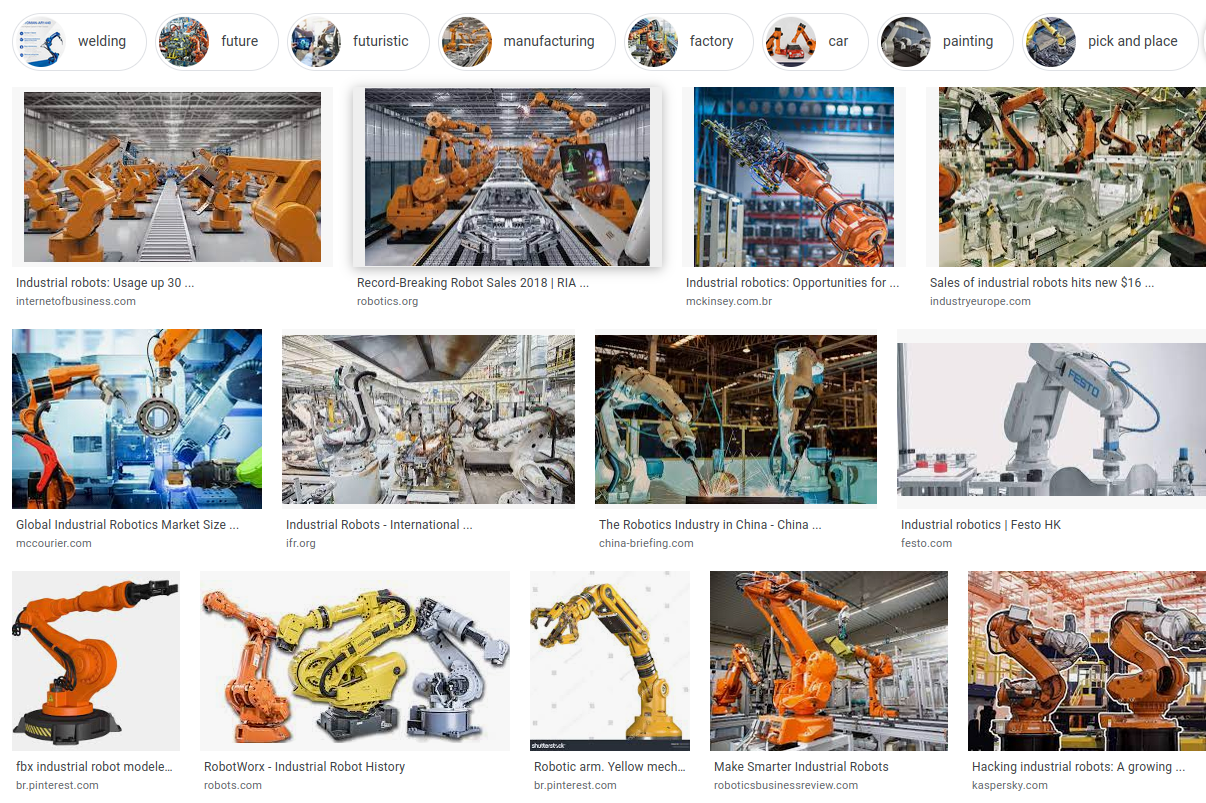
\includegraphics[width=0.6\textwidth]{./images/industrialrobots.png}}
        {https://www.google.com/search?q=Industrial+robot}
    \end{block}
    \href{https://www.youtube.com/watch?v=fn3KWM1kuAw}{\faPlay (Do You Love Me?)}
\end{frame}


\begin{frame}{Modern Robots}
	\framesubtitle{\textcolor{blue}{Robots Change the Way We Work!}}
	\begin{center}
        \cpright{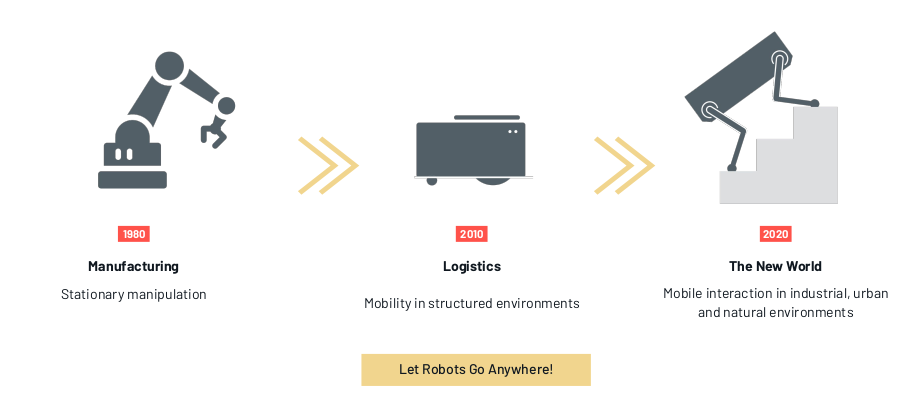
\includegraphics[width=0.8\textwidth]{./images/robots_evolution.png}}
        {https://www.google.com/search?q=Industrial+robot}
    \end{center}

\end{frame}


\begin{frame}{Modern Robots}
	\framesubtitle{\textcolor{blue}{Robots Change the Way We Work!} - 
    \textcolor{purple}{Collaborative Robots}}
	\begin{center}
        \cpright{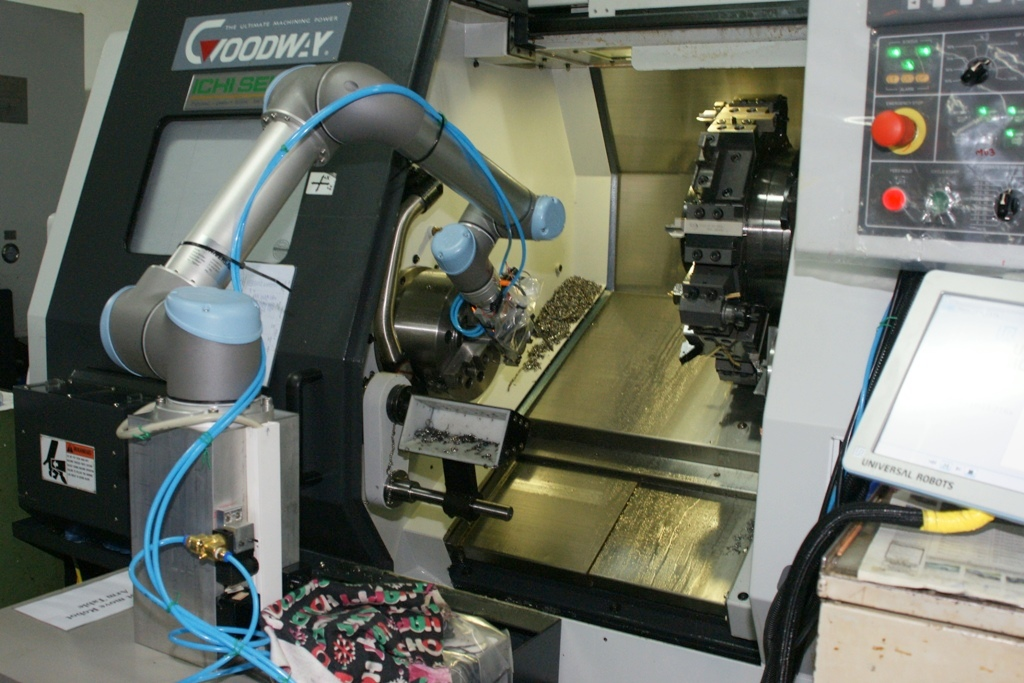
\includegraphics[width=0.45\textwidth]{./images/cobots1.jpg}}
        {https://www.universal-robots.com/}
        \cpright{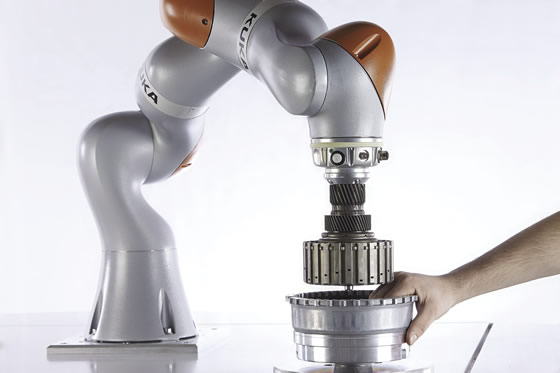
\includegraphics[width=0.45\textwidth]{./images/cobots2.jpeg}}
        {https://www.kuka.com/}
    \end{center}
    \href {https://www.youtube.com/watch?v=PtncirKiBXQ}{\faPlay(COBOTS) }
\end{frame}

\begin{frame}{Modern Robots}
	\framesubtitle{\textcolor{blue}{Robots Change the Way We Work!}}
	\begin{center}
        \cpright{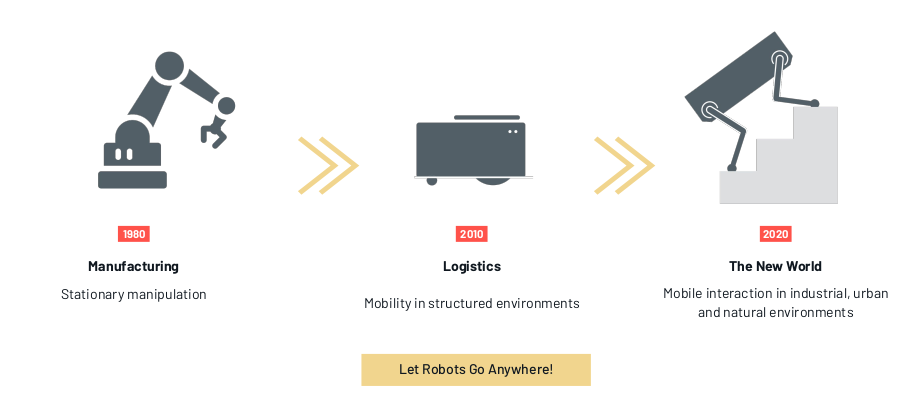
\includegraphics[width=0.8\textwidth]{./images/robots_evolution.png}}
        {https://www.google.com/search?q=Industrial+robot}
    \end{center}

    \href {https://www.youtube.com/watch?v=24jufNhuUSI}{\faPlay(Spot - NYPD) }
    \href {https://www.youtube.com/watch?v=QpJBmkOpp1Q}{\faPlay(ANYmalC - Vale) }
\end{frame}


\begin{frame}[fragile]{Modern Robots}
	\framesubtitle{\textcolor{purple}{ANYmal C} - Case-Based Learning}

	\begin{minipage}{0.5\textwidth}
        \cpright{\href{https://www.anybotics.com/anymal-legged-robot/}
        {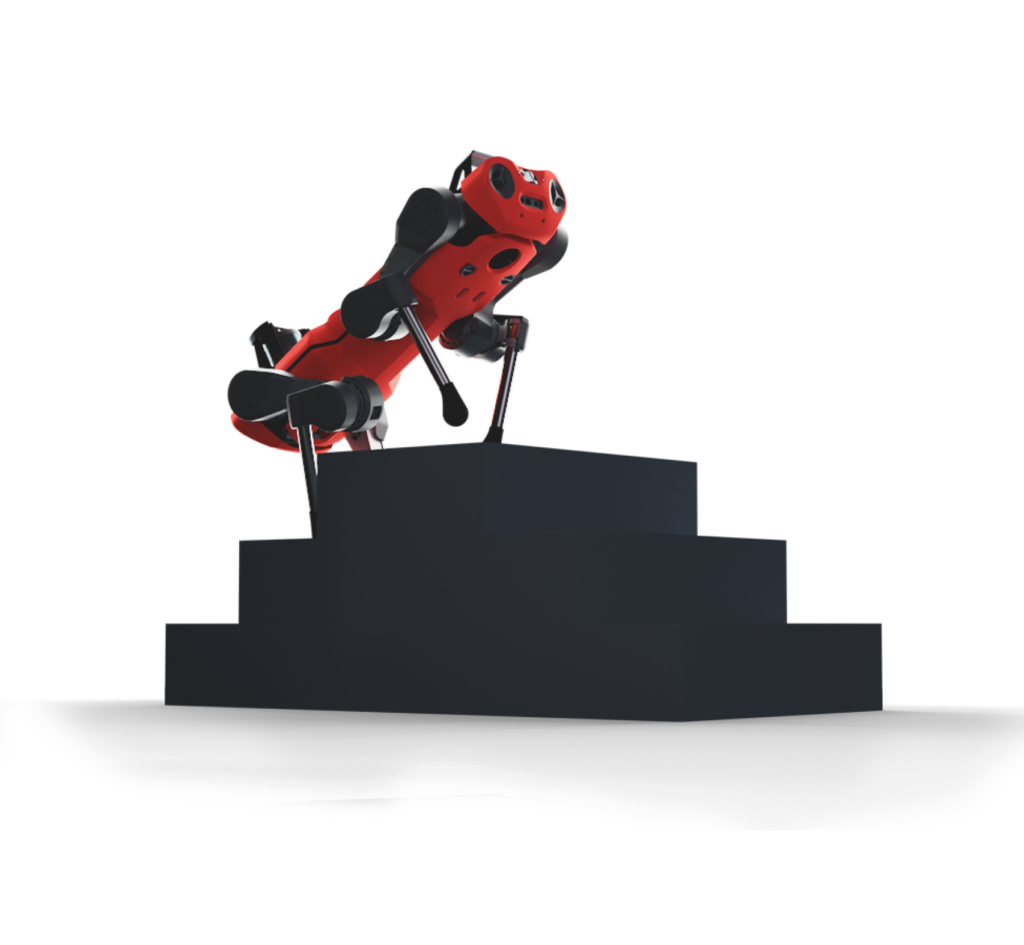
\includegraphics[width=1\textwidth]{./images/ANYmal.png}}}
        {https://www.anybotics.com/anymal-legged-robot/}
    \end{minipage}
    \begin{minipage}{0.5\textwidth}
        \begin{itemize}
            \item \textcolor{purple}{\textbf{Advanced Sensing}}:
            \begin{itemize}
                \item Obstacle Detection;
                \item Environment Scanning;
                \item Wide-Angle Cameras;
                \item GPS
            \end{itemize}
            \item \textcolor{purple}{\textbf{Full autonomy}}:
            \begin{itemize}
                \item Autonomous Path Planning;
                \item Obstacle Avoidance;
                \item Real-Time Motion Planning;
                \item Human Detection (WIP)
            \end{itemize}
            \item \textcolor{purple}{\textbf{Docking station}}:
            \begin{itemize}
                \item Battery run time: $> 2h$;
                \item For full charge:  $3h$;
            \end{itemize}
            \item \textcolor{purple}{\textbf{Ease of use}}:
            \begin{itemize}
                \item Joystick;
                \item Workstation;
            \end{itemize}
        \end{itemize}
    \end{minipage}
\end{frame}

\begin{frame}[c]{Modern Robots}
	\framesubtitle{\textcolor{purple}{ANYmal C} - Evolution}
    \vspace{0.1in}
    \cpright{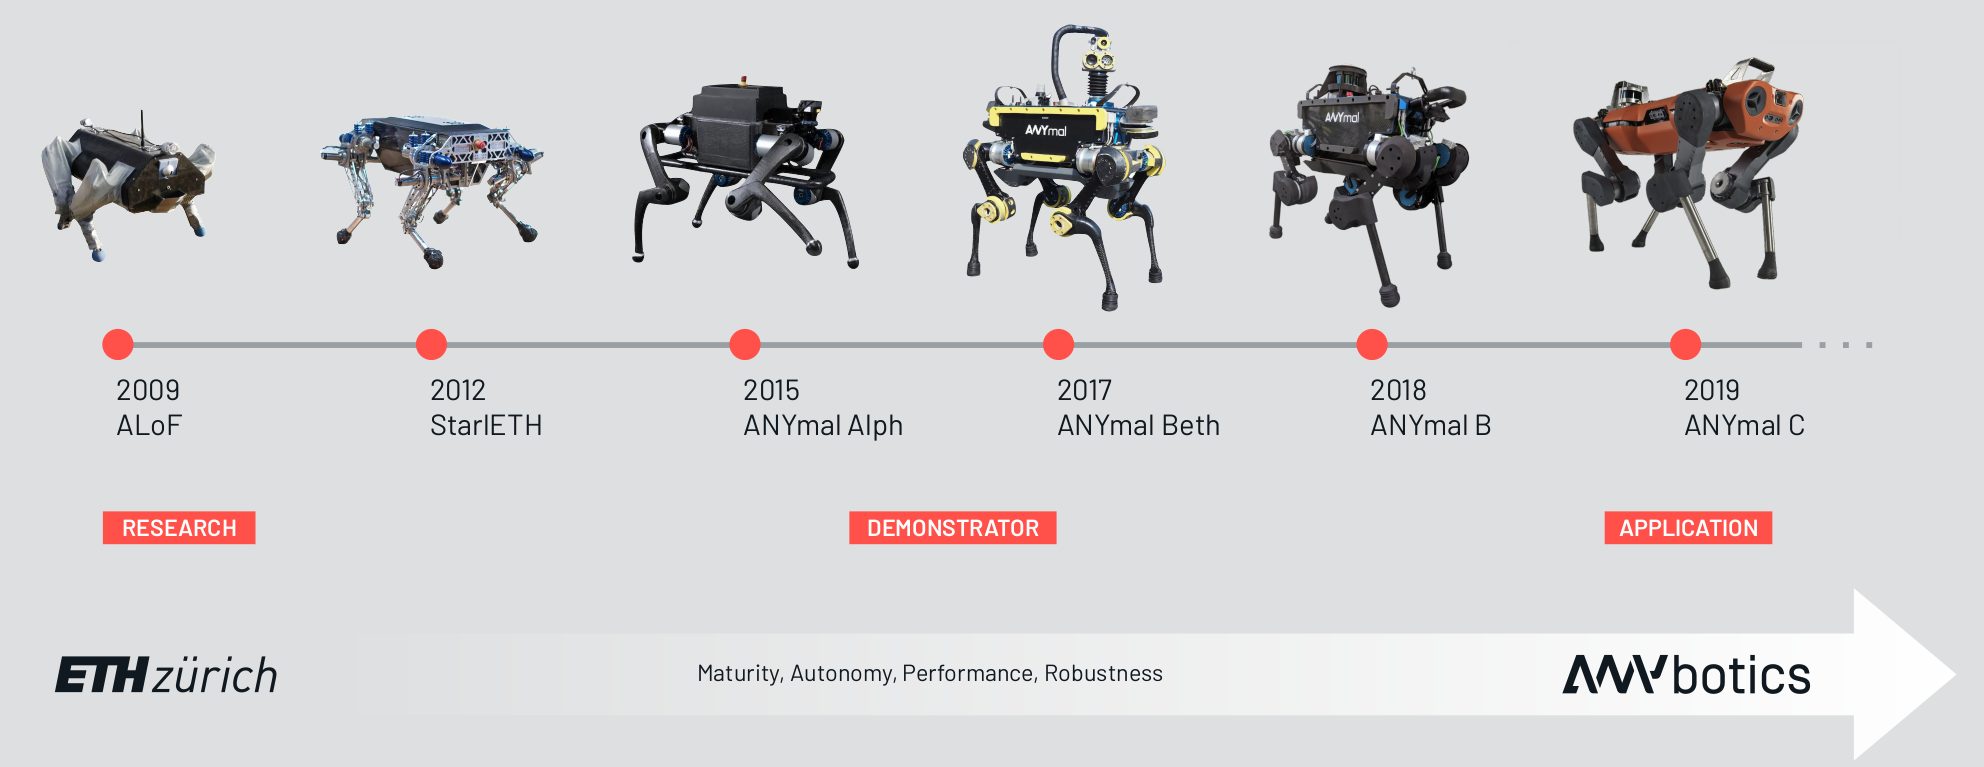
\includegraphics[width=1\textwidth]{./images/eth_ANYmal.png}}
    {https://www.anybotics.com/anymal-legged-robot/}

\end{frame}

\begin{frame}[c]{Modern Robots}
	\framesubtitle{\textcolor{purple}{ANYmal C} - Sensors}
    \vspace{0.1in}
    \cpright{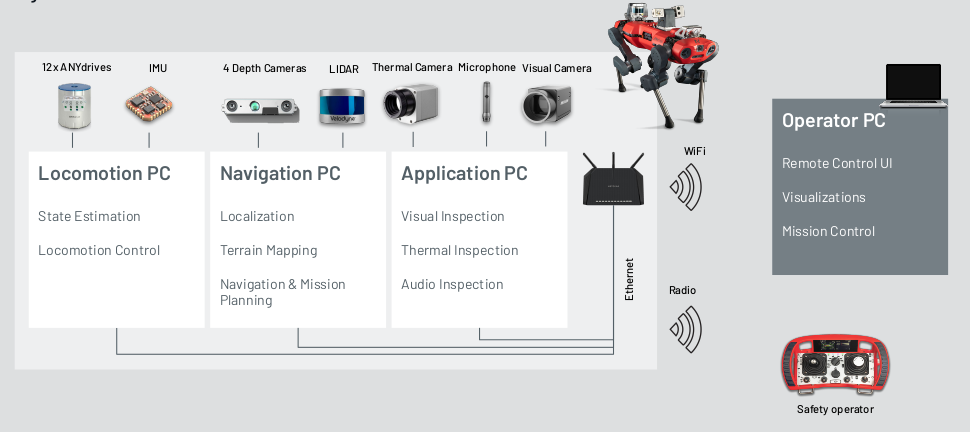
\includegraphics[width=1\textwidth]{./images/ANYmal_sensores.png}}
    {https://www.anybotics.com/anymal-legged-robot/}
\end{frame}

\begin{frame}[fragile]{Modern Robots}
	\framesubtitle{\textcolor{purple}{ANYmal C} - AnyDrive - Brushless DC Motor}
	\begin{minipage}{0.3\textwidth}
        \cpright{\href{https://www.anybotics.com/anymal-legged-robot/}
        {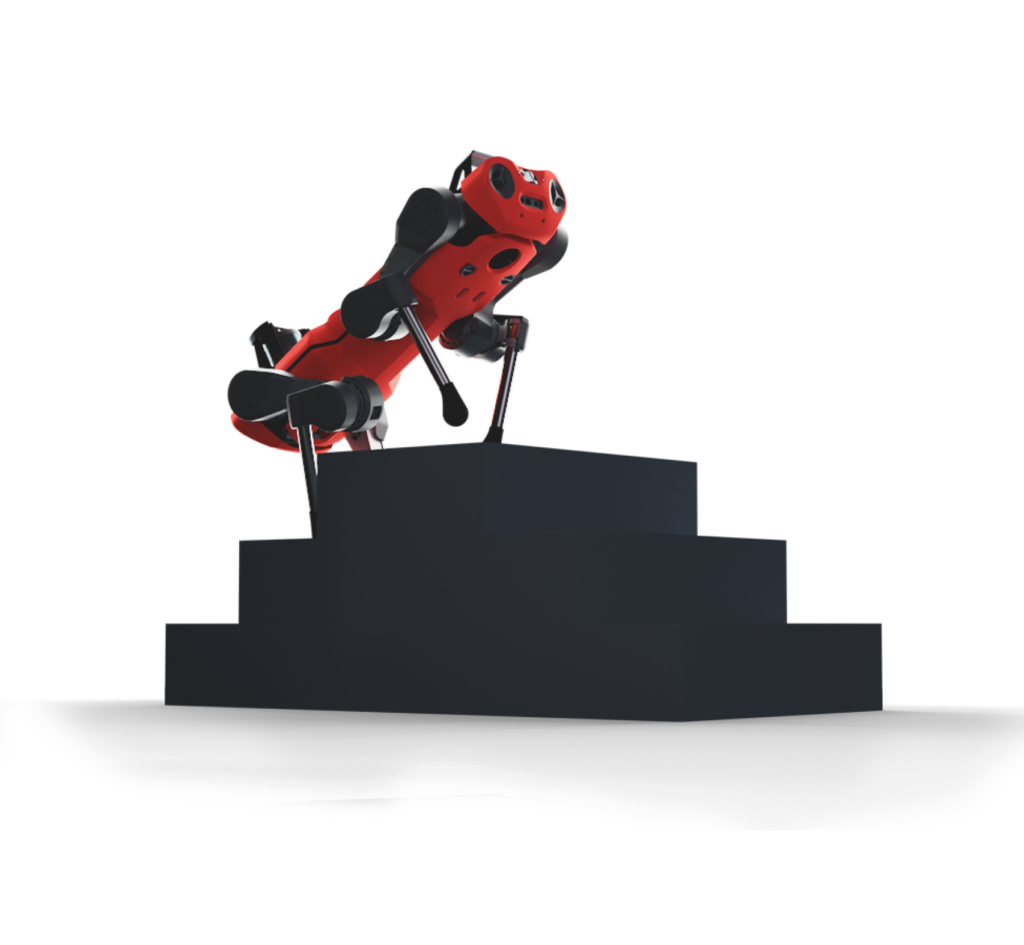
\includegraphics[width=1\textwidth]{./images/ANYmal.png}}}
        {https://www.anybotics.com/anymal-legged-robot/}
    \end{minipage}
    \begin{minipage}{0.7\textwidth}
        \textcolor{purple}{\textbf{AnyDrive - Brushless DC Motor}}:
        \begin{itemize}
                \item  A powerful brushless motor, a backlash-free gear, high-precision encoders, and efficient power electronics
            \end{itemize}
            \begin{figure}
                \cpright{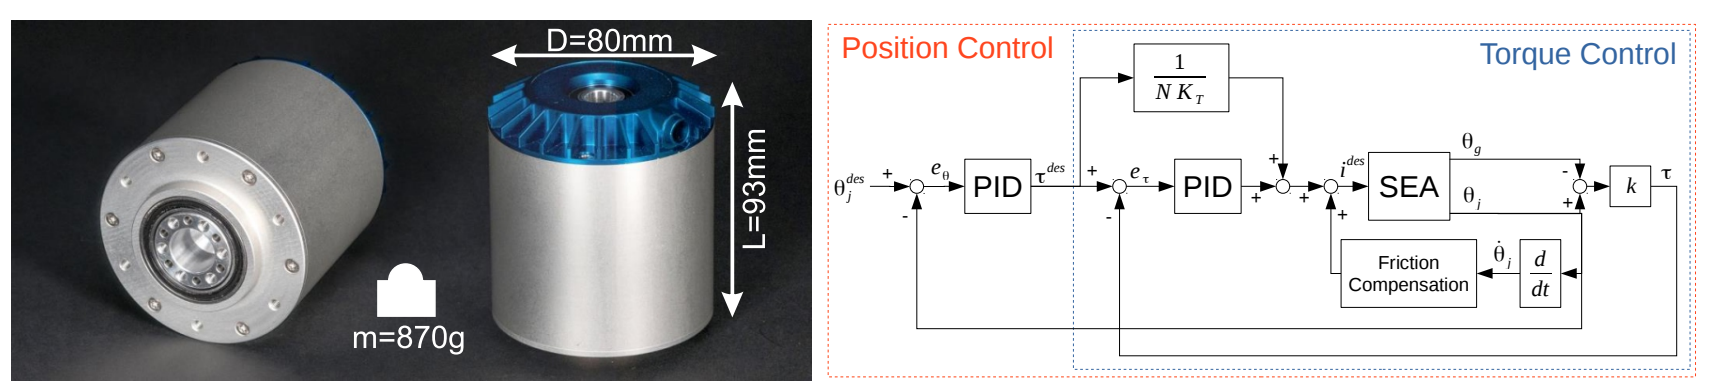
\includegraphics[width=1\textwidth]{./images/ANYDrive.png}}
                {\cite{noauthor_anydrive}}
                \caption{ANYdrive: Compact, compliant joint units for advanced interaction}
            \end{figure}
            
    \end{minipage}
\end{frame}


\begin{frame}[fragile]{Modern Robots}
	\framesubtitle{\textcolor{purple}{ANYmal C} - IMU Sensors}
	\begin{minipage}{0.3\textwidth}
        \cpright{\href{https://www.anybotics.com/anymal-legged-robot/}
        {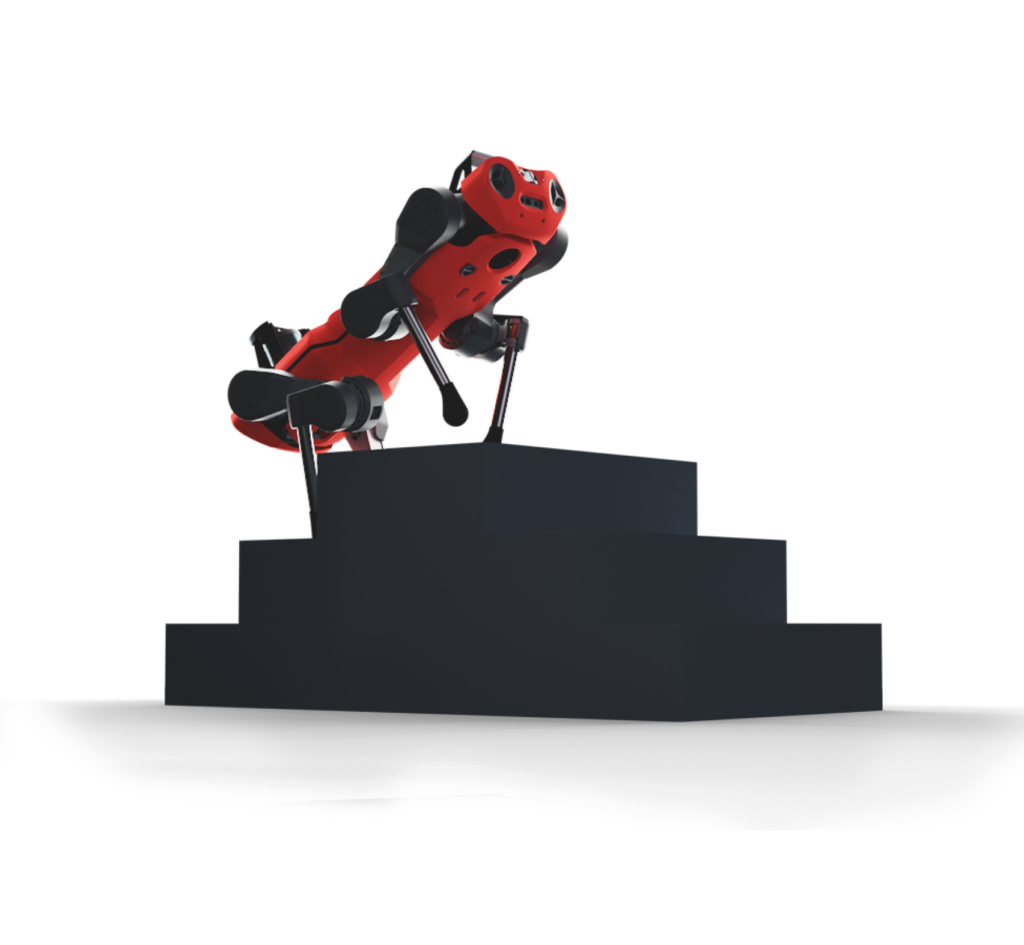
\includegraphics[width=1\textwidth]{./images/ANYmal.png}}}
        {https://www.anybotics.com/anymal-legged-robot/}
    \end{minipage}
    \begin{minipage}{0.7\textwidth}
        \textcolor{purple}{\textbf{IMU ([I]nertial [M]easurement [U]nit)}}:
        \begin{itemize}
                \item An inertial measurement unit (IMU) is a device that uses gyroscopes and accelerometers to
                estimate the relative position, velocity, and acceleration of a moving vehicle.
            \end{itemize}
            \cpright{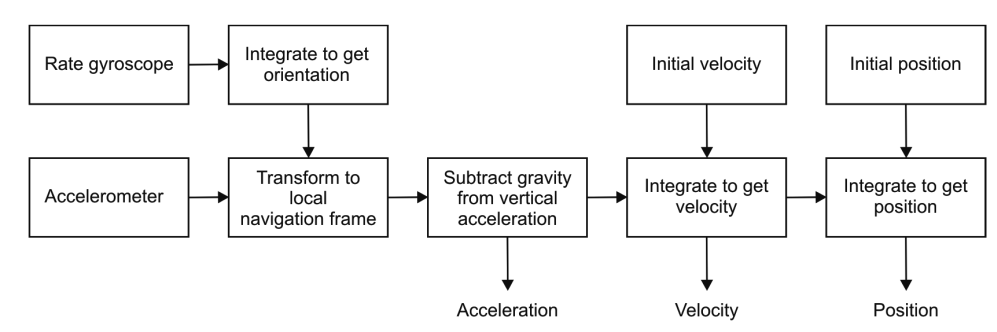
\includegraphics[width=1\textwidth]{./images/anyIMU.png}}
            {\cite{siegwart2011introduction}}
    \end{minipage}
\end{frame}

\begin{frame}[fragile]{Modern Robots}
	\framesubtitle{\textcolor{purple}{ANYmal C} - IMU Sensors}
	\begin{minipage}{0.3\textwidth}
        \cpright{\href{https://www.anybotics.com/anymal-legged-robot/}
        {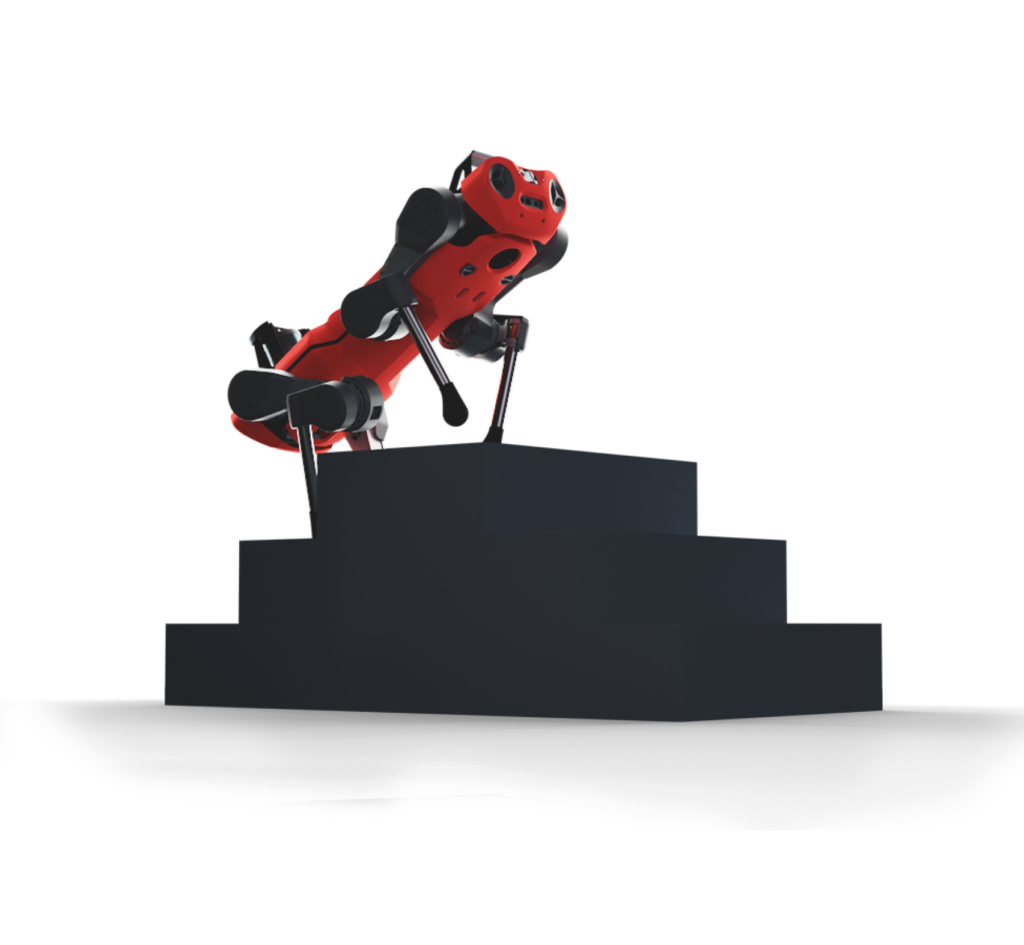
\includegraphics[width=1\textwidth]{./images/ANYmal.png}}}
        {https://www.anybotics.com/anymal-legged-robot/}
    \end{minipage}
    \begin{minipage}{0.7\textwidth}
            \textcolor{purple}{\textbf{IMU ([I]nertial [M]easurement [U]nit)}}:
            \begin{itemize}
                \item Modern accelerometers and gyroscopes are often small [M]icro [E]lectro-[M]echanical [S]ystems (MEMS);
            \end{itemize}
            \begin{figure}
                \cpright{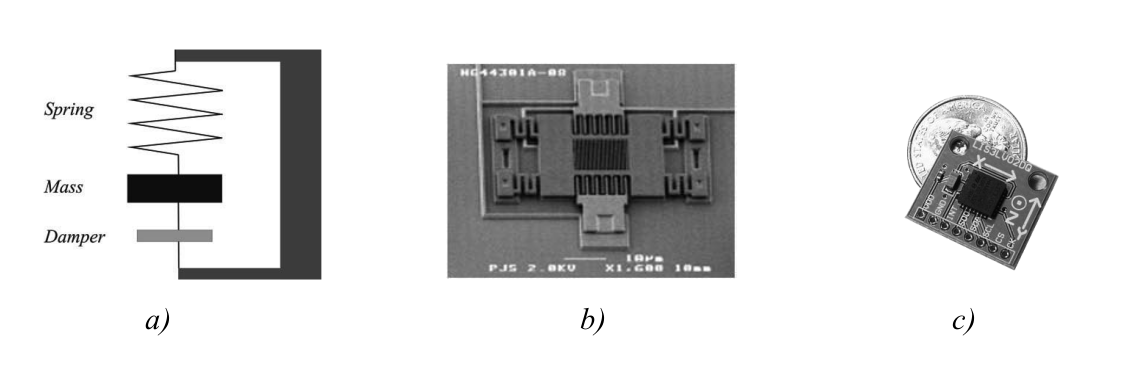
\includegraphics[width=1\textwidth]{./images/anyIMEMS.png}}
                {\cite{siegwart2011introduction}}
                \caption{(a) Working principle; (b) An example MEMS accelerometer; (c) An example commercial MEMS accelerometer.}
            \end{figure}
    \end{minipage}
\end{frame}


\begin{frame}[fragile]{Modern Robots}
	\framesubtitle{\textcolor{purple}{ANYmal C} - IMU LIDAR}
	\begin{minipage}{0.3\textwidth}
        \cpright{\href{https://www.anybotics.com/anymal-legged-robot/}
        {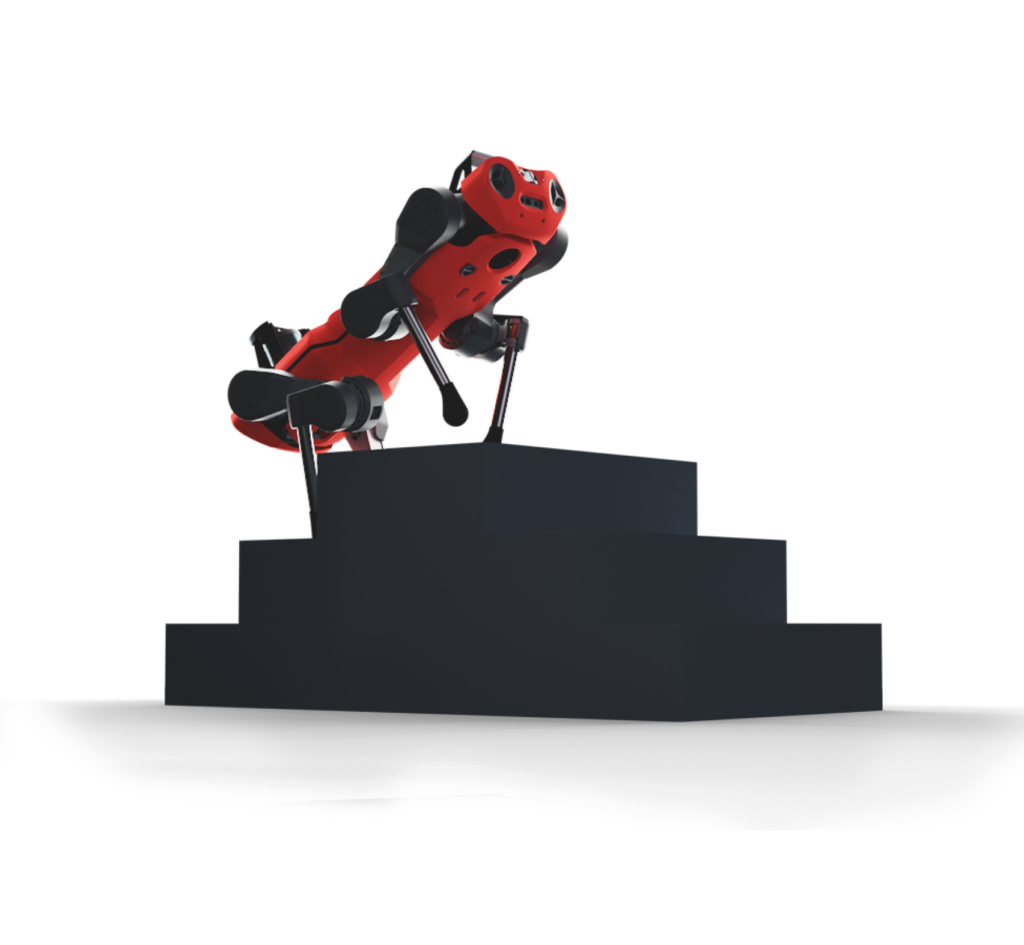
\includegraphics[width=1\textwidth]{./images/ANYmal.png}}}
        {https://www.anybotics.com/anymal-legged-robot/}
    \end{minipage}
    \begin{minipage}{0.7\textwidth}
            \textcolor{purple}{\textbf{LIDAR ([LI]ght [D]etection [A]nd [R]anging)}}:
            \begin{itemize}
                \item LIDAR devices produce a range estimate based on the time needed for the light to reach the target and return.
            \end{itemize}
            \begin{figure}
                \cpright{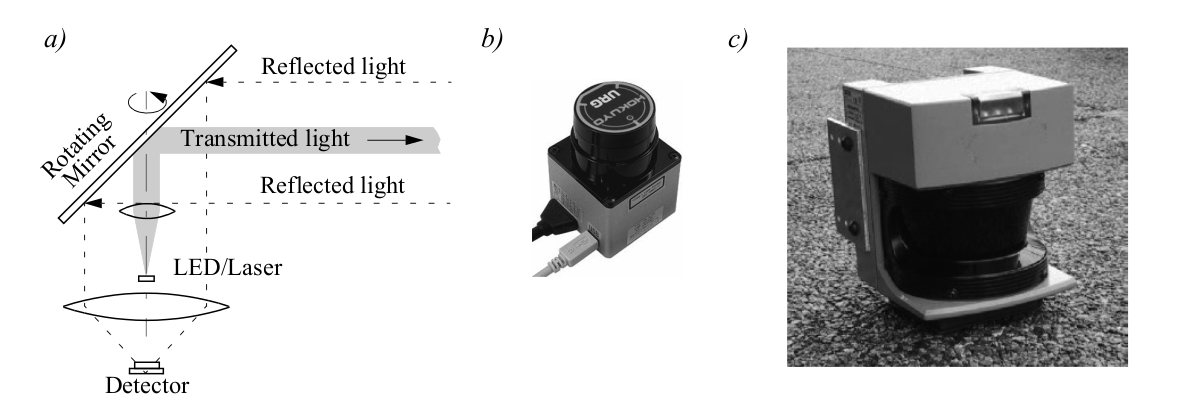
\includegraphics[width=0.9\textwidth]{./images/ANYmal_LIDAR.png}}
                {\cite{siegwart2011introduction}}
                \caption{(a) Schematic drawing of laser range sensor; (b) 240-degree laser rangefinder; (c) Industrial 180 degree laser range sensor.}
            \end{figure}
    \end{minipage}
\end{frame}


\begin{frame}[fragile]{Modern Robots}
	\framesubtitle{\textcolor{purple}{ANYmal C} - IMU LIDAR}
	\begin{minipage}{0.3\textwidth}
        \cpright{\href{https://www.anybotics.com/anymal-legged-robot/}
        {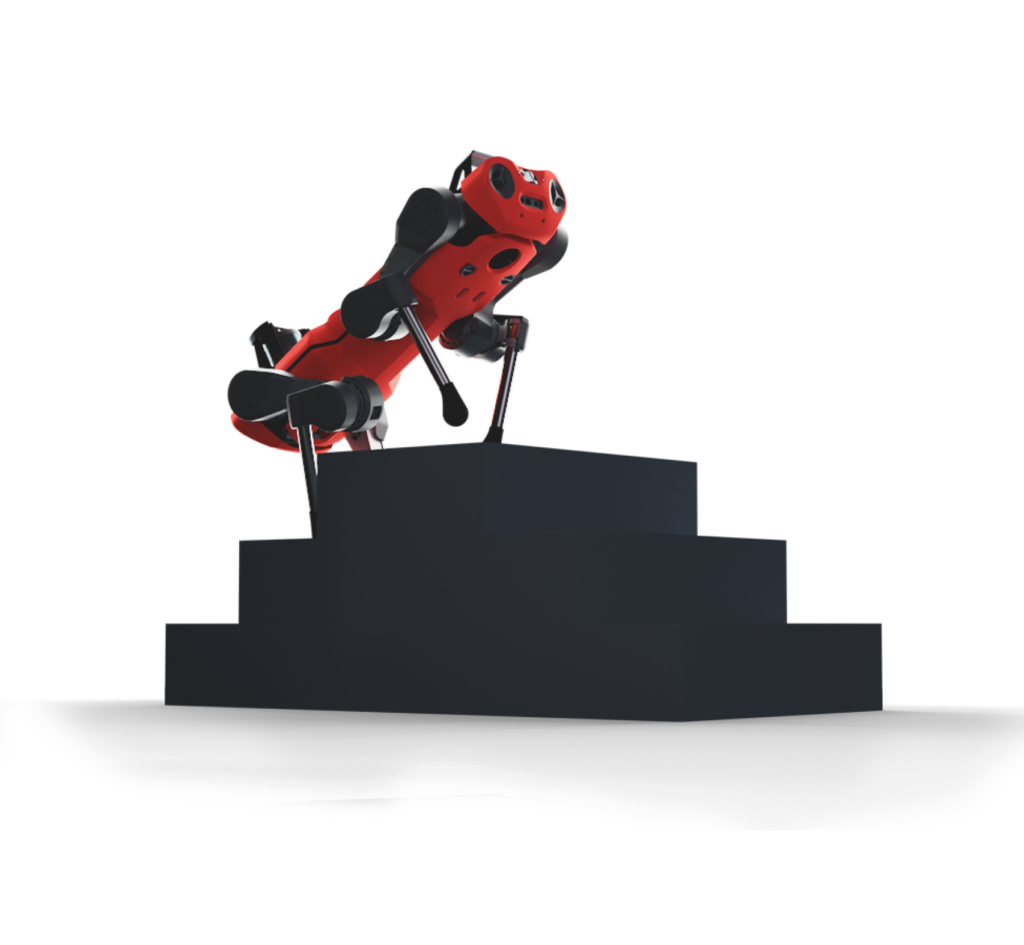
\includegraphics[width=1\textwidth]{./images/ANYmal.png}}}
        {https://www.anybotics.com/anymal-legged-robot/}
    \end{minipage}
    \begin{minipage}{0.7\textwidth}
            \textcolor{purple}{\textbf{LIDAR ([LI]ght [D]etection [A]nd [R]anging)}}:
            \begin{itemize}
                \item LIDAR devices produce a range estimate based on the time needed for the light to reach the target and return.
            \end{itemize}
            \begin{figure}
                \cpright{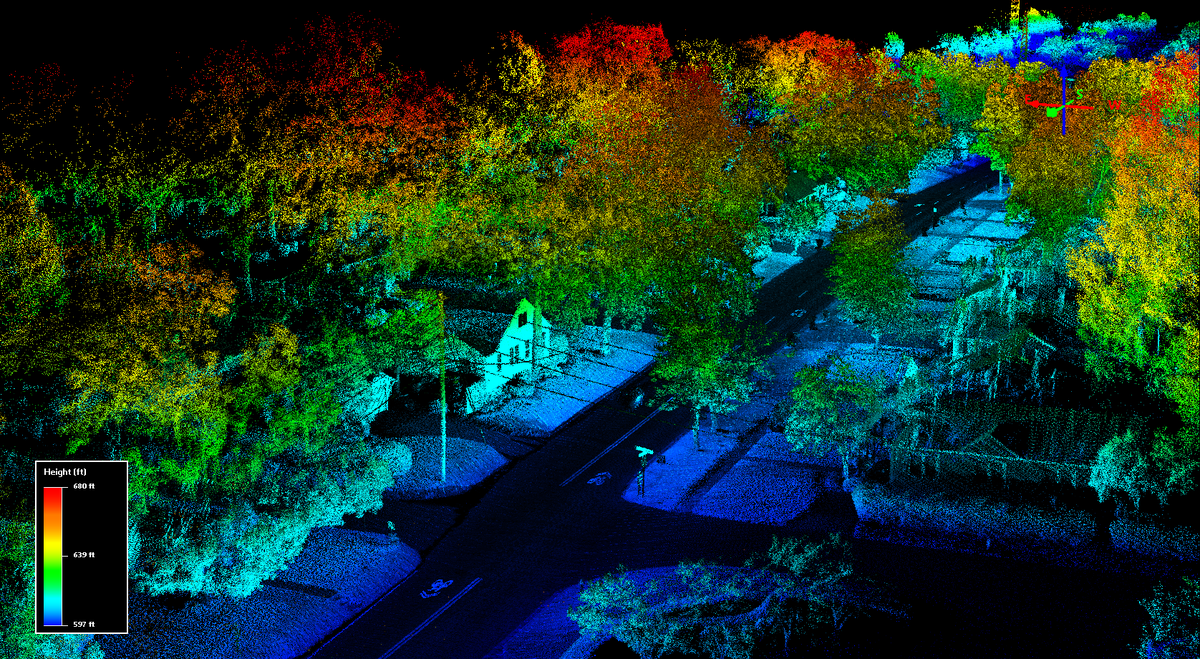
\includegraphics[width=0.9\textwidth]{./images/blackmore-lidar.png}}
                {https://www.zdnet.com/article/am-vs-fm-the-battle-brewing-in-lidar-technology/}
                \caption{Street Map Example.}
            \end{figure}
    \end{minipage}
\end{frame}

\begin{frame}[fragile]{Modern Robots}
	\framesubtitle{\textcolor{purple}{ANYmal C} - Stereo Cameras}
	\begin{minipage}{0.3\textwidth}
        \cpright{\href{https://www.anybotics.com/anymal-legged-robot/}
        {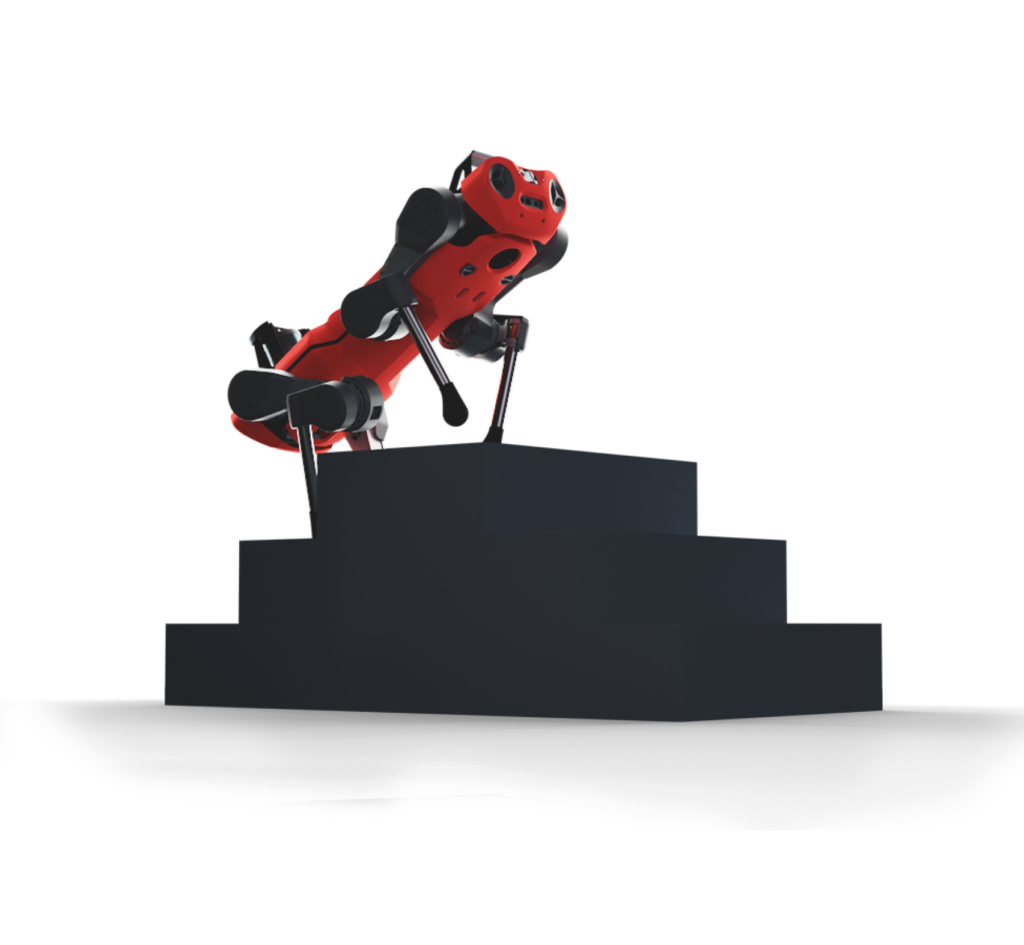
\includegraphics[width=1\textwidth]{./images/ANYmal.png}}}
        {https://www.anybotics.com/anymal-legged-robot/}
    \end{minipage}
    \begin{minipage}{0.7\textwidth}
            \textcolor{purple}{\textbf{Stereo Cameras}}:
            \begin{itemize}
                \item Distance information can be computed using two cameras that are mounted in a fixed distance.
            \end{itemize}
            \begin{figure}
                \cpright{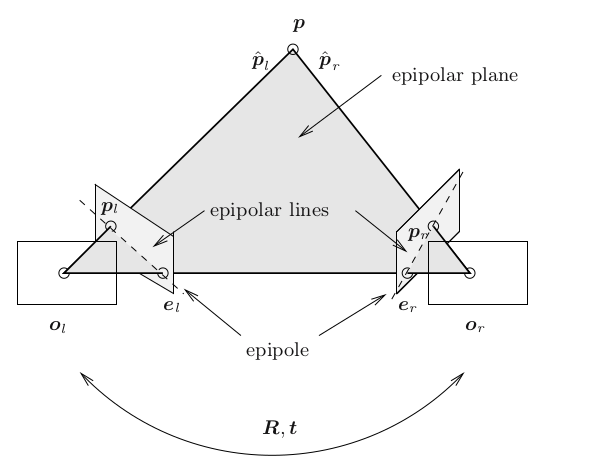
\includegraphics[width=0.5\textwidth]{./images/stereo_cam.png}}
                {\cite{nuchter20083d}}
                \caption{General stereo geometry.}
            \end{figure}
    \end{minipage}
\end{frame}



\begin{frame}[fragile]{Modern Robots}
	\framesubtitle{\textcolor{purple}{ANYmal C} - Stereo Cameras}
	\begin{minipage}{0.3\textwidth}
        \cpright{\href{https://www.anybotics.com/anymal-legged-robot/}
        {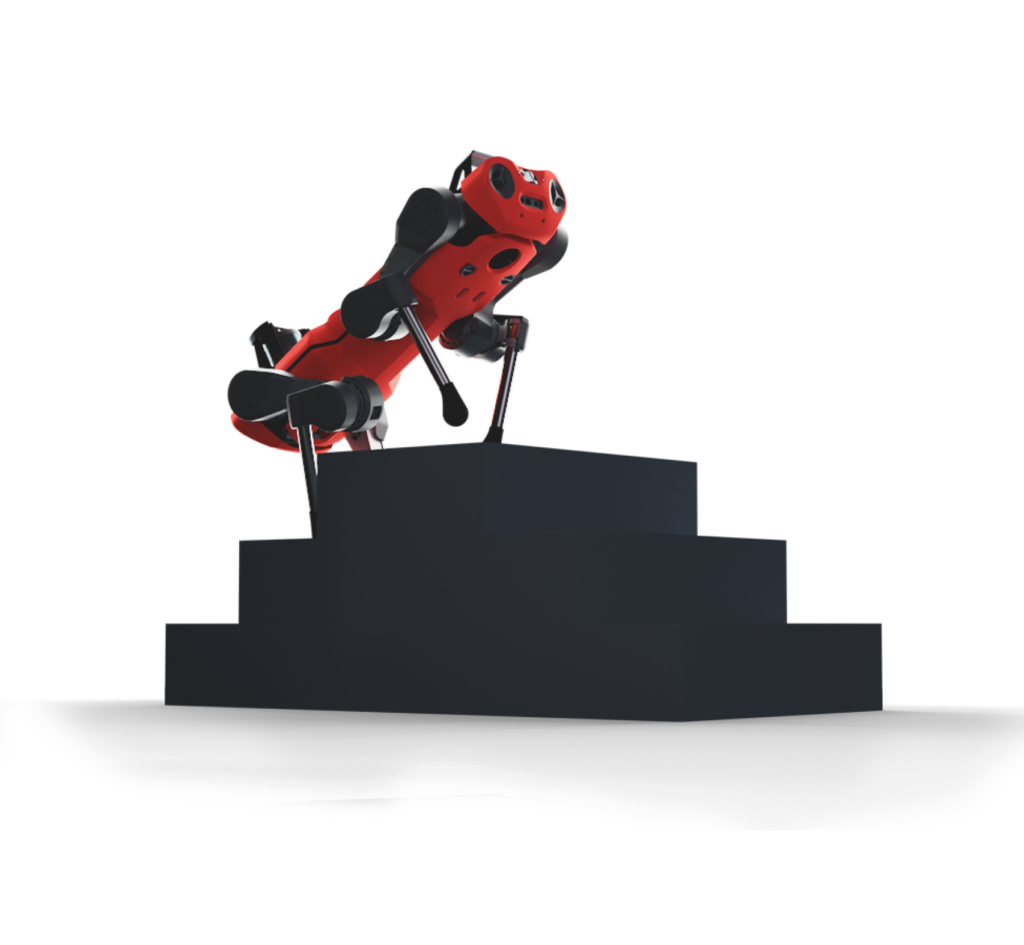
\includegraphics[width=1\textwidth]{./images/ANYmal.png}}}
        {https://www.anybotics.com/anymal-legged-robot/}
    \end{minipage}
    \begin{minipage}{0.7\textwidth}
            \textcolor{purple}{\textbf{Stereo Cameras}}:
            \begin{itemize}
                \item Distance information can be computed using two cameras that are mounted in a fixed distance.
            \end{itemize}
            \begin{figure}
                \cpright{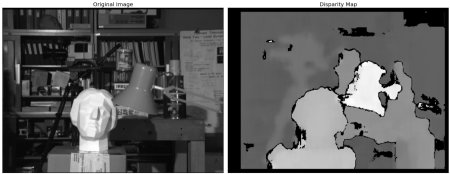
\includegraphics[width=0.8\textwidth]{./images/disparity_map.jpg}}
                {\cite{opencv_library}\footnote{\textbf{More info:} \href{https://opencv-python-tutroals.readthedocs.io/en/latest/py_tutorials/py_calib3d/py_depthmap/py_depthmap.html}{OpenCV: Depth Map from Stereo Images}}}
                \caption{original image (left) and its disparity map (right).}
            \end{figure}
    \end{minipage}
\end{frame}

\begin{frame}[fragile]{Modern Robots}
	\framesubtitle{\textcolor{purple}{ANYmal C} - Structured Light Depth Cameras}
	\begin{minipage}{0.3\textwidth}
        \cpright{\href{https://www.anybotics.com/anymal-legged-robot/}
        {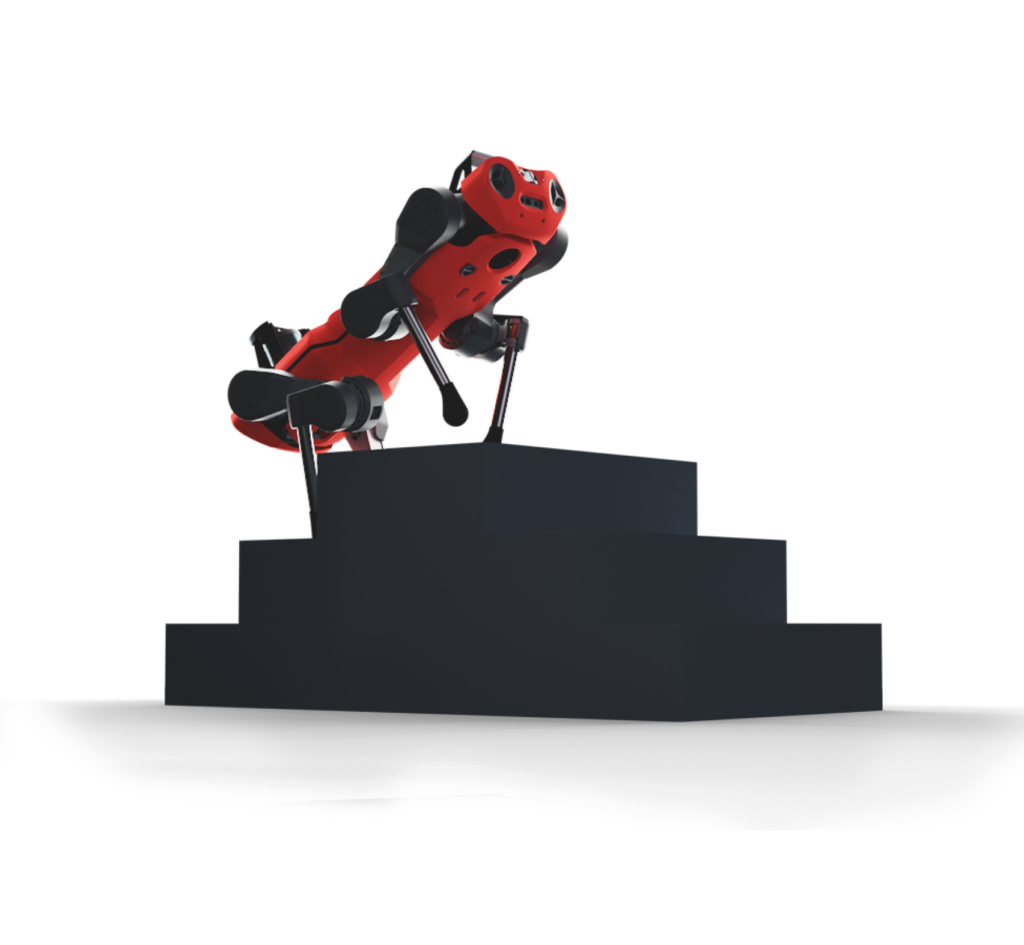
\includegraphics[width=1\textwidth]{./images/ANYmal.png}}}
        {https://www.anybotics.com/anymal-legged-robot/}
    \end{minipage}
    \begin{minipage}{0.7\textwidth}
            \textcolor{purple}{\textbf{Structured Light Depth Cameras}}:
            \begin{itemize}
                \item In Structured light depth camera systems there is a \textit{light projectors} or \textit{illuminators}, devices in which each pixel $p_A$ illuminates a scene point $P$ by its specific light value thus creating a spatial pattern.
            \end{itemize}
            \begin{figure}
                \cpright{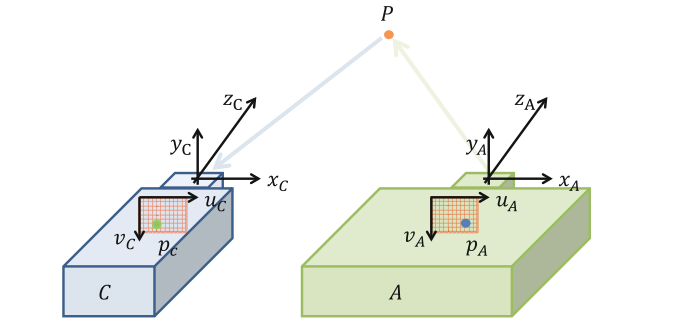
\includegraphics[width=0.5\textwidth]{./images/depth_cam.png}}
                {\cite{zanuttigh2016time}}
                \caption{Active triangulation by a system made of a camera $C$ and a light projector $A$.}
            \end{figure}
    \end{minipage}
    \href {https://www.zivid.com/3d-point-cloud-examples/}{\faPlay(ZIVID) }
\end{frame}


\begin{frame}[fragile]{Modern Robots}
	\framesubtitle{\textcolor{purple}{ANYmal C} - Structured Light Depth Cameras}
	\begin{minipage}{0.3\textwidth}
        \cpright{\href{https://www.anybotics.com/anymal-legged-robot/}
        {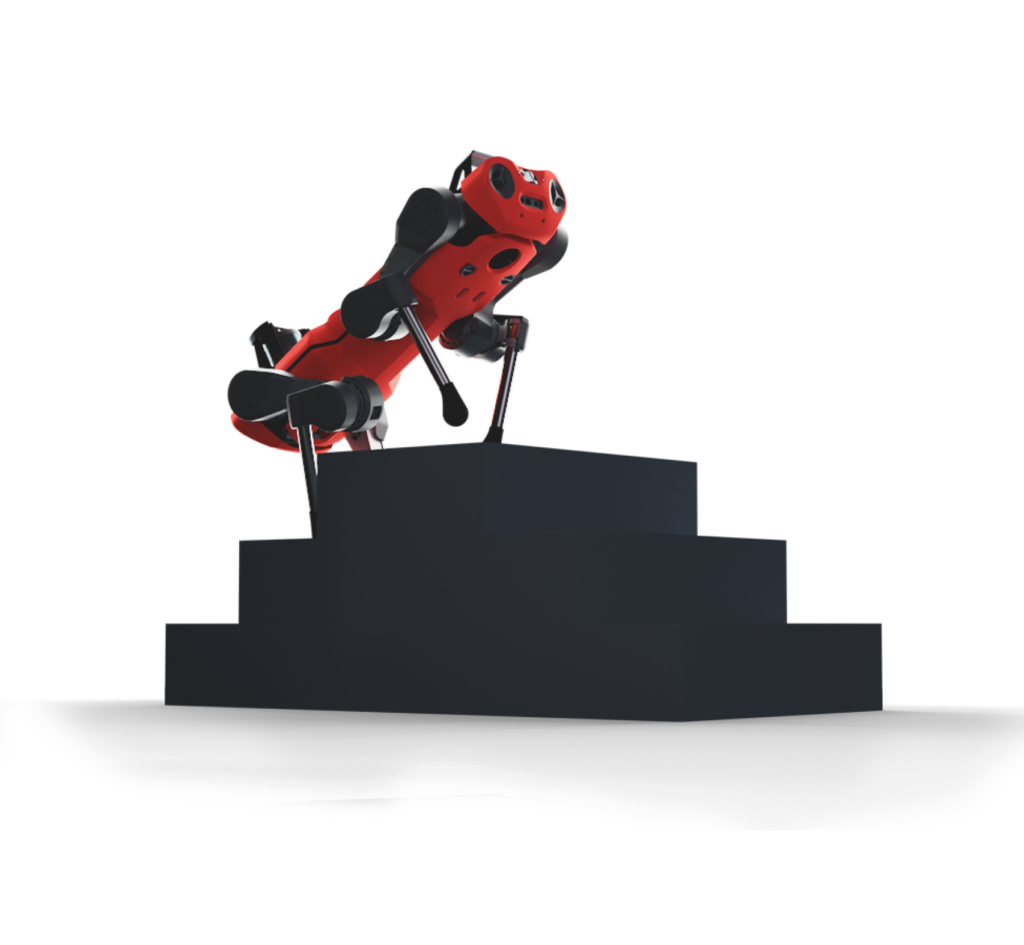
\includegraphics[width=1\textwidth]{./images/ANYmal.png}}}
        {https://www.anybotics.com/anymal-legged-robot/}
    \end{minipage}
    \begin{minipage}{0.7\textwidth}
            \textcolor{purple}{\textbf{Structured Light Depth Cameras}}:
            \begin{itemize}
                \item In Structured light depth camera systems there is a \textit{light projectors} or \textit{illuminators}, devices in which each pixel $p_A$ illuminates a scene point $P$ by its specific light value thus creating a spatial pattern.
            \end{itemize}
            \begin{figure}
                \cpright{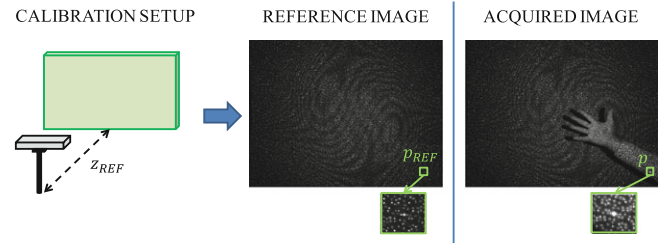
\includegraphics[width=0.8\textwidth]{./images/depth_cam_ex.png}}
                {\cite{zanuttigh2016time}}
                \caption{Illustration of the reference image usage}
            \end{figure}
    \end{minipage}
\end{frame}

\begin{frame}[fragile]{Modern Robots}
	\framesubtitle{\textcolor{purple}{ANYmal C} - Structured Light Depth Cameras}
	\begin{minipage}{0.3\textwidth}
        \cpright{\href{https://www.anybotics.com/anymal-legged-robot/}
        {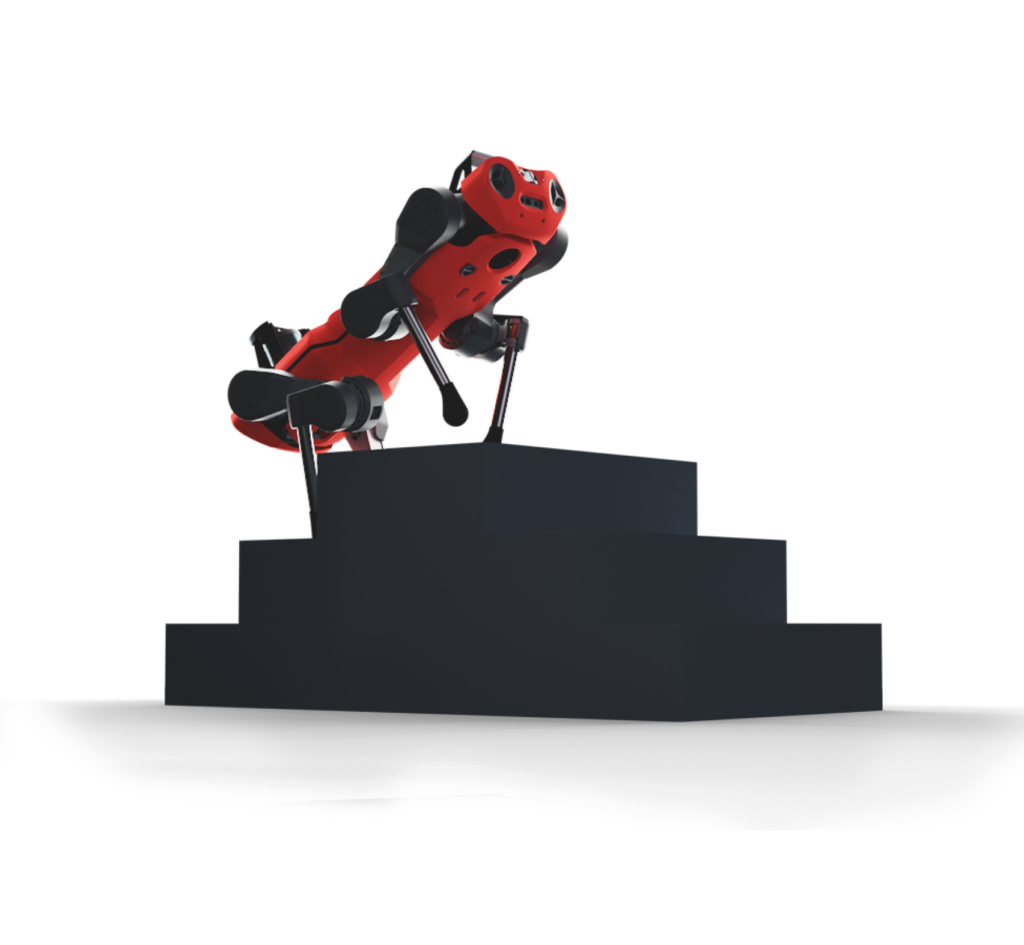
\includegraphics[width=1\textwidth]{./images/ANYmal.png}}}
        {https://www.anybotics.com/anymal-legged-robot/}
    \end{minipage}
    \begin{minipage}{0.7\textwidth}
            \textcolor{purple}{\textbf{Structured Light Depth Cameras}}:
            \begin{itemize}
                \item In Structured light depth camera systems there is a \textit{light projectors} or \textit{illuminators}.
            \end{itemize}
            \begin{figure}
                \cpright{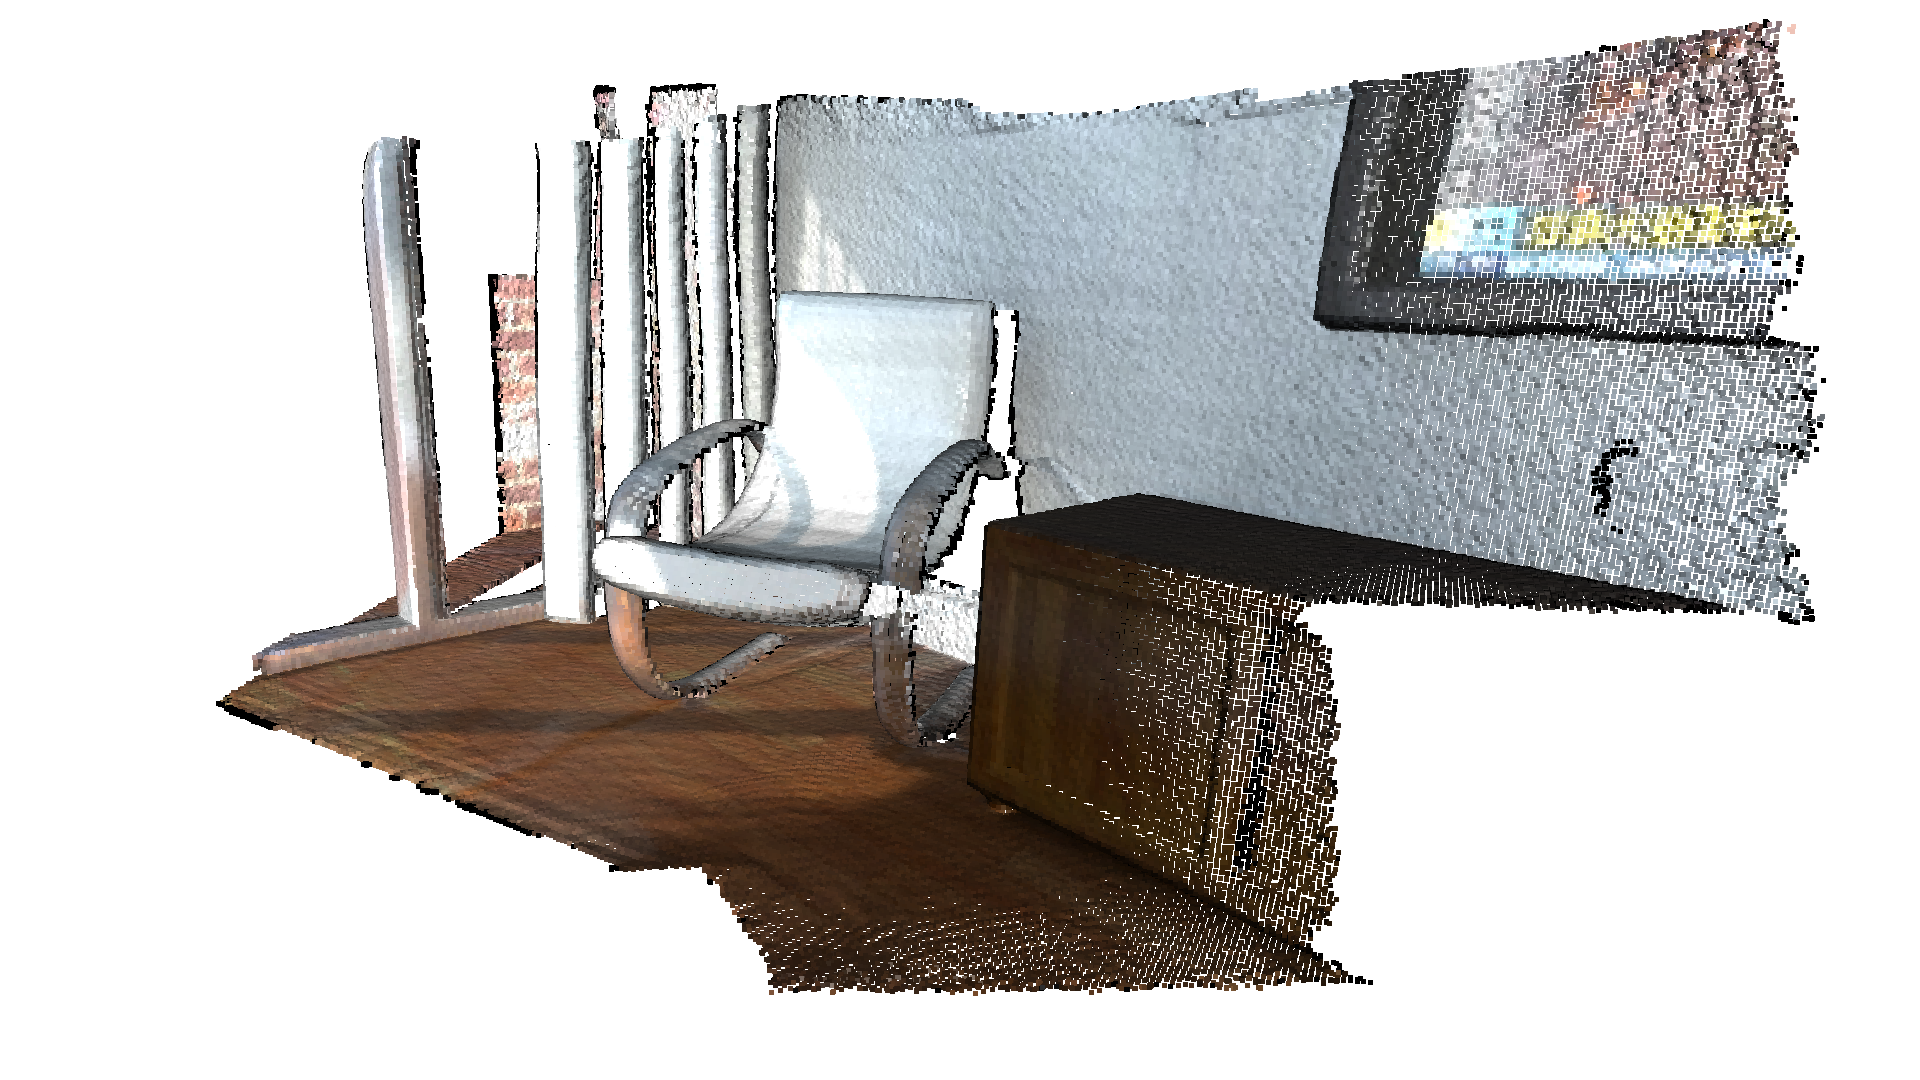
\includegraphics[width=0.6\textwidth]{./images/open3d_example.png}}
                {\cite{Zhou2018}\footnote{\textbf{More info:} \href{http://www.open3d.org/docs/release/tutorial/visualization/visualization.html}{Open3D: Visualization }}}
                \caption{Illustration of the reference image usage}
            \end{figure}
    \end{minipage}
\end{frame}


\begin{frame}[fragile]{Modern Robots}
	\framesubtitle{\textcolor{purple}{ANYmal C} - Simulation}
	\begin{minipage}{0.3\textwidth}
        \cpright{\href{https://www.anybotics.com/anymal-legged-robot/}
        {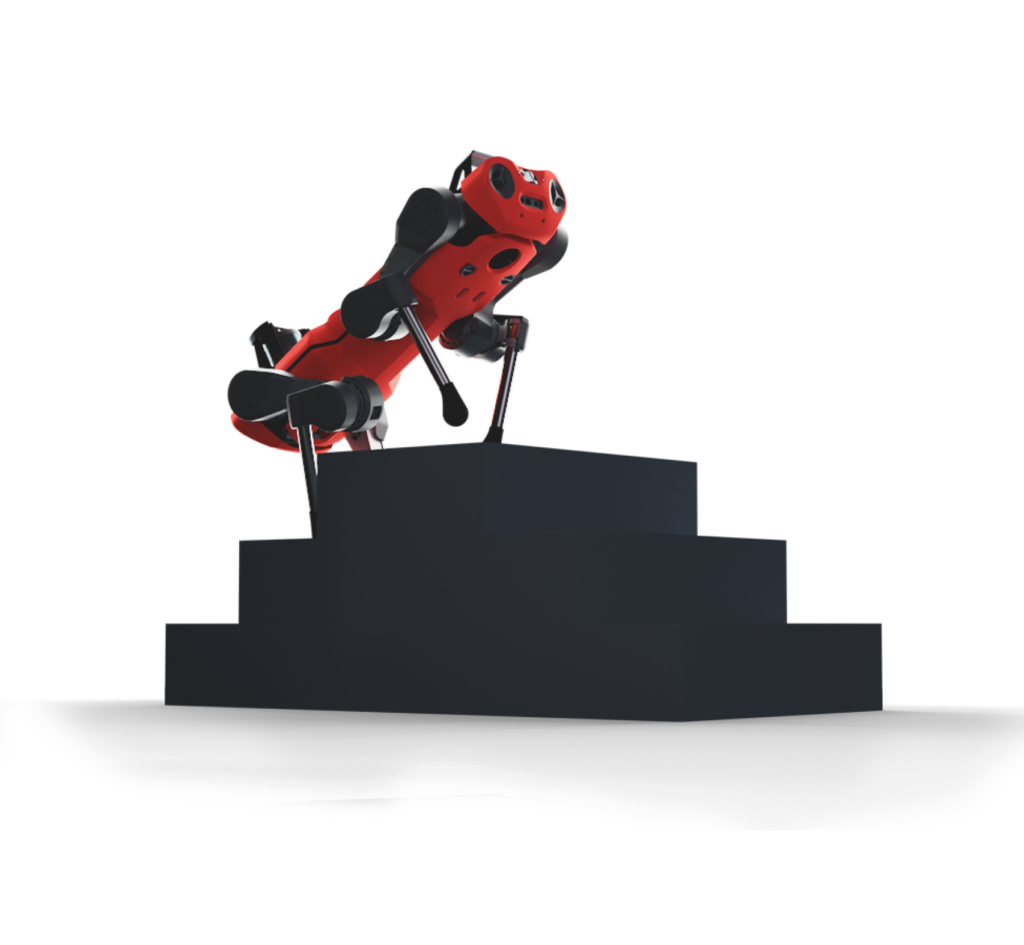
\includegraphics[width=1\textwidth]{./images/ANYmal.png}}}
        {https://www.anybotics.com/anymal-legged-robot/}
    \end{minipage}
    \begin{minipage}{0.7\textwidth}
            \textcolor{purple}{\textbf{Simulation - ROS (Robot Operating System)}}:
            \begin{itemize}
                \item Robot State Simulation, Visualization and Interaction.
            \end{itemize}
            \begin{figure}
                \cpright{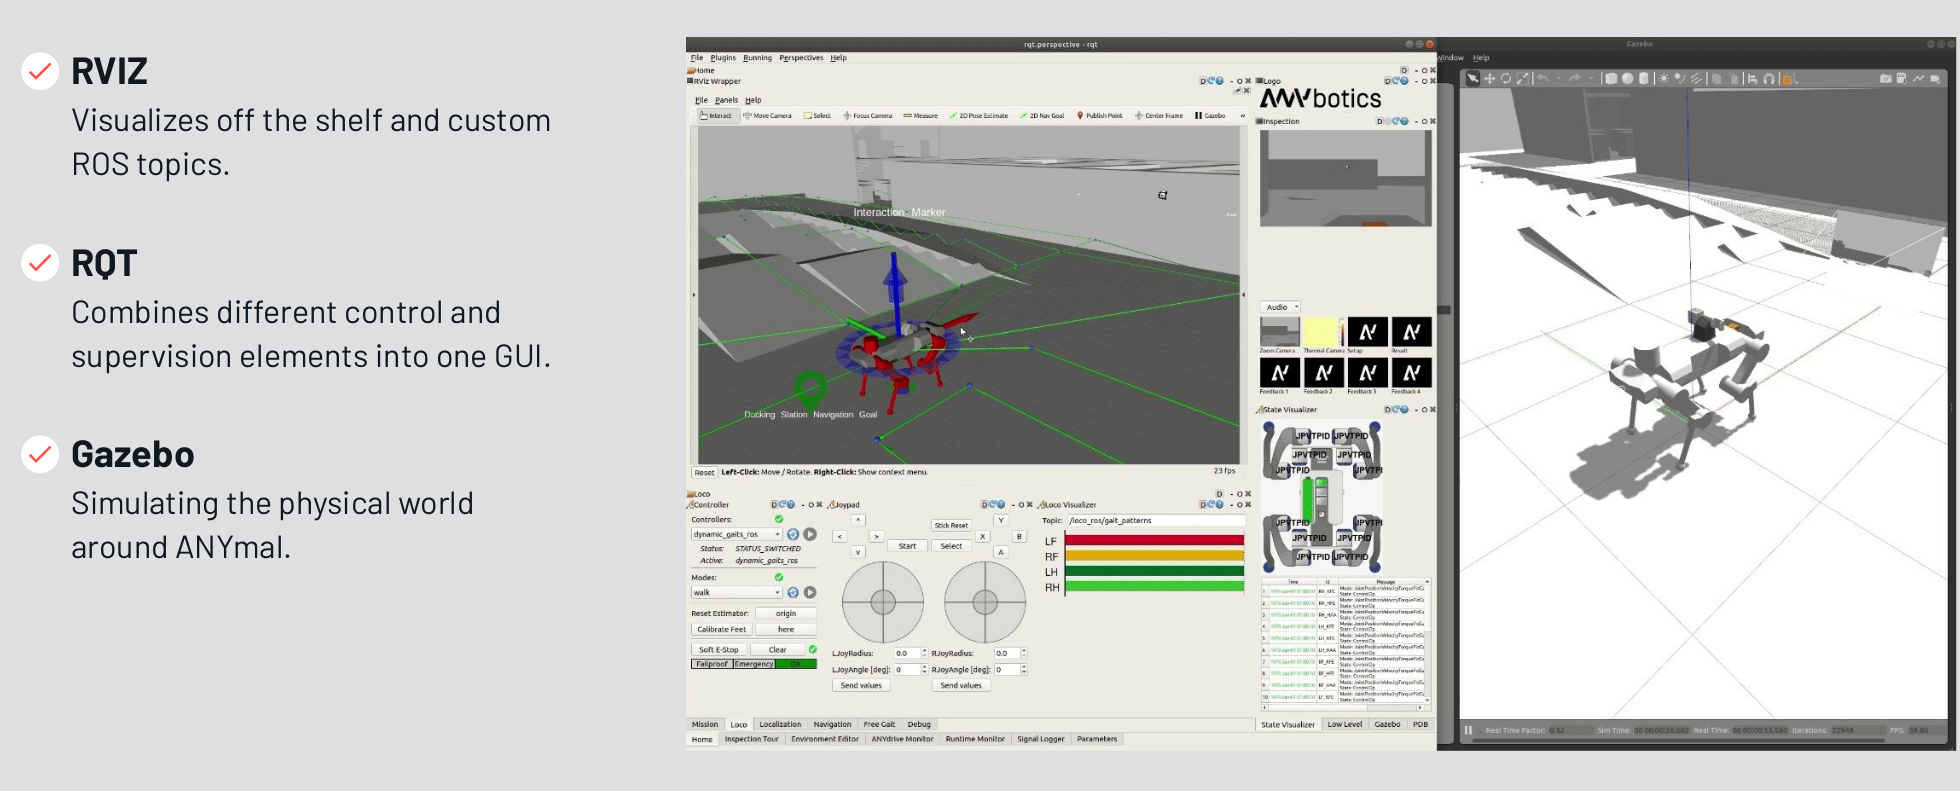
\includegraphics[width=1\textwidth]{./images/ANYmal_ROS.png}}
                {https://www.anybotics.com/anymal-legged-robot/}
            \end{figure}
    \end{minipage}
\end{frame}


\begin{frame}[fragile]{Modern Robots}
	\framesubtitle{\textcolor{purple}{ANYmal C} - Real Robot}
	\begin{minipage}{0.3\textwidth}
        \cpright{\href{https://www.anybotics.com/anymal-legged-robot/}
        {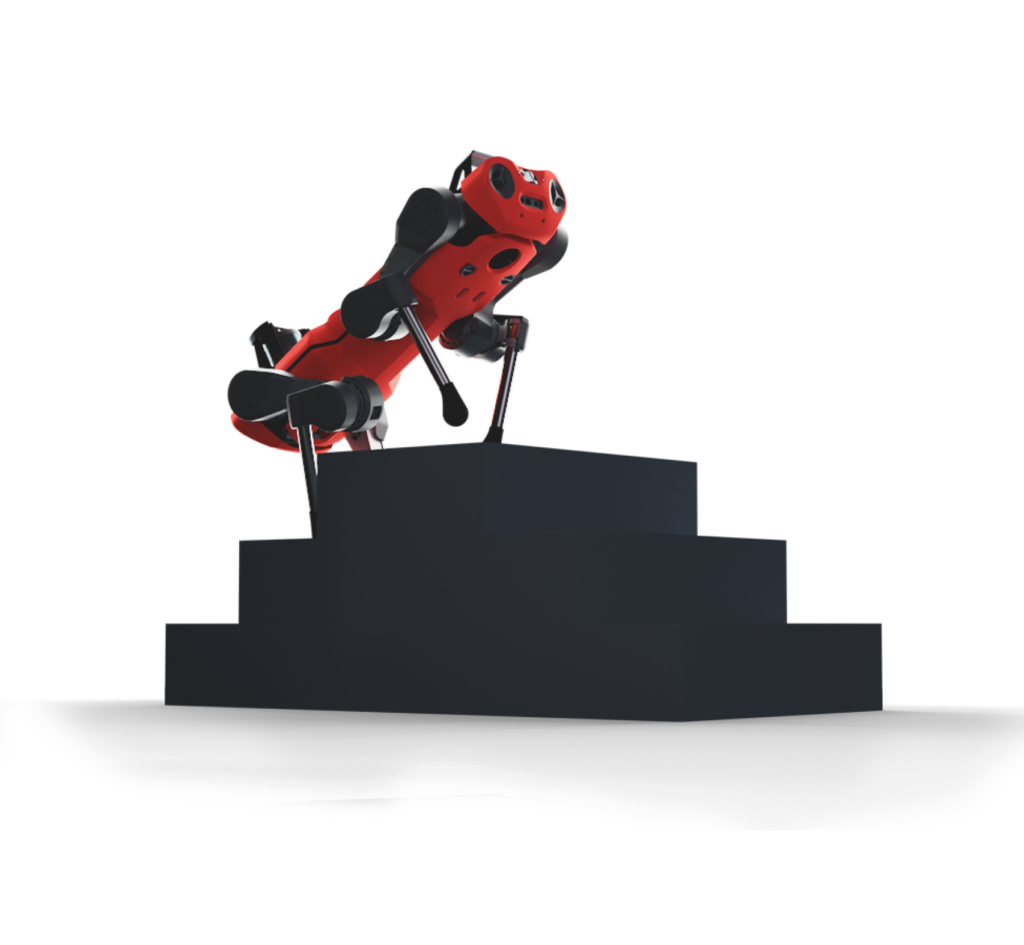
\includegraphics[width=1\textwidth]{./images/ANYmal.png}}}
        {https://www.anybotics.com/anymal-legged-robot/}
    \end{minipage}
    \begin{minipage}{0.7\textwidth}
            \textcolor{purple}{\textbf{Real Robot}}:
            \begin{itemize}
                \item Interaction with Real Robot.
            \end{itemize}
            \begin{figure}
                \cpright{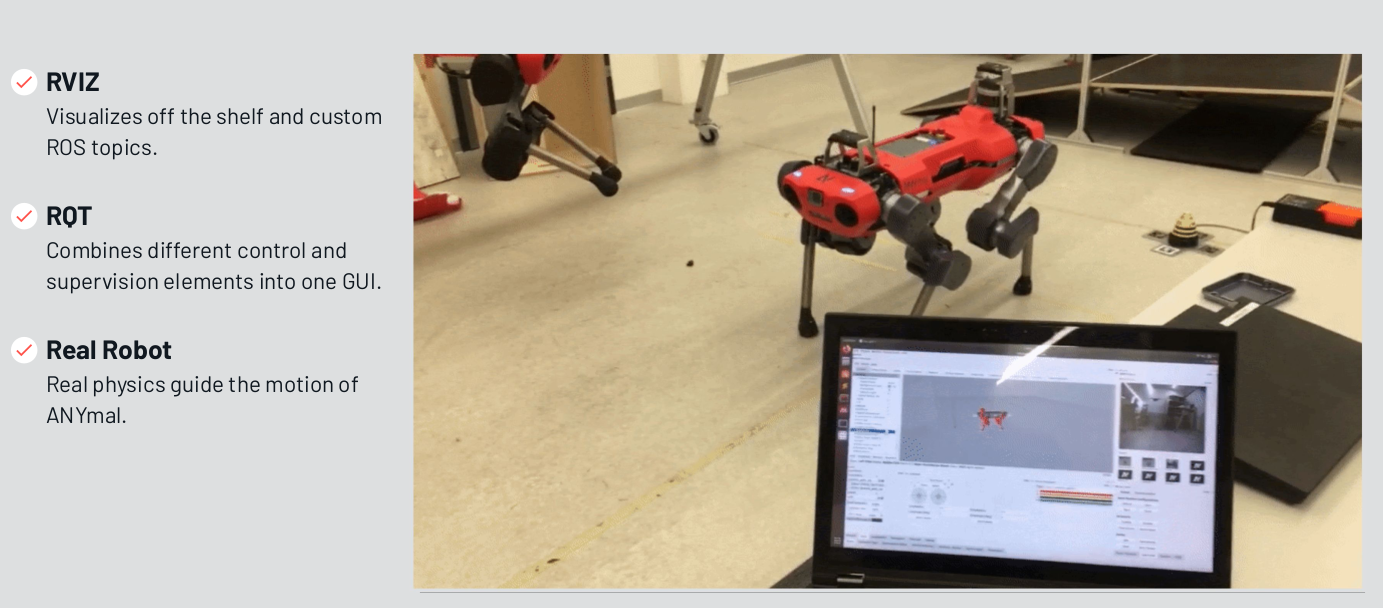
\includegraphics[width=0.99\textwidth]{./images/ANYmal_ROS_real.png}}
                {https://www.anybotics.com/anymal-legged-robot/}
            \end{figure}
    \end{minipage}
    \href{https://leggedrobotics.github.io/rl-blindloco/}{\small(ANYmal Learning to walk)}
    \href{https://www.youtube.com/watch?v=lKYh6uuCwRY}{\small(\faPlay Learning to walk)}
\end{frame}


\begin{frame}[fragile]{Modern Robots}
	\framesubtitle{\textcolor{purple}{ANYmal C} - Real Robot}
	\begin{minipage}{0.3\textwidth}
        \cpright{\href{https://www.anybotics.com/anymal-legged-robot/}
        {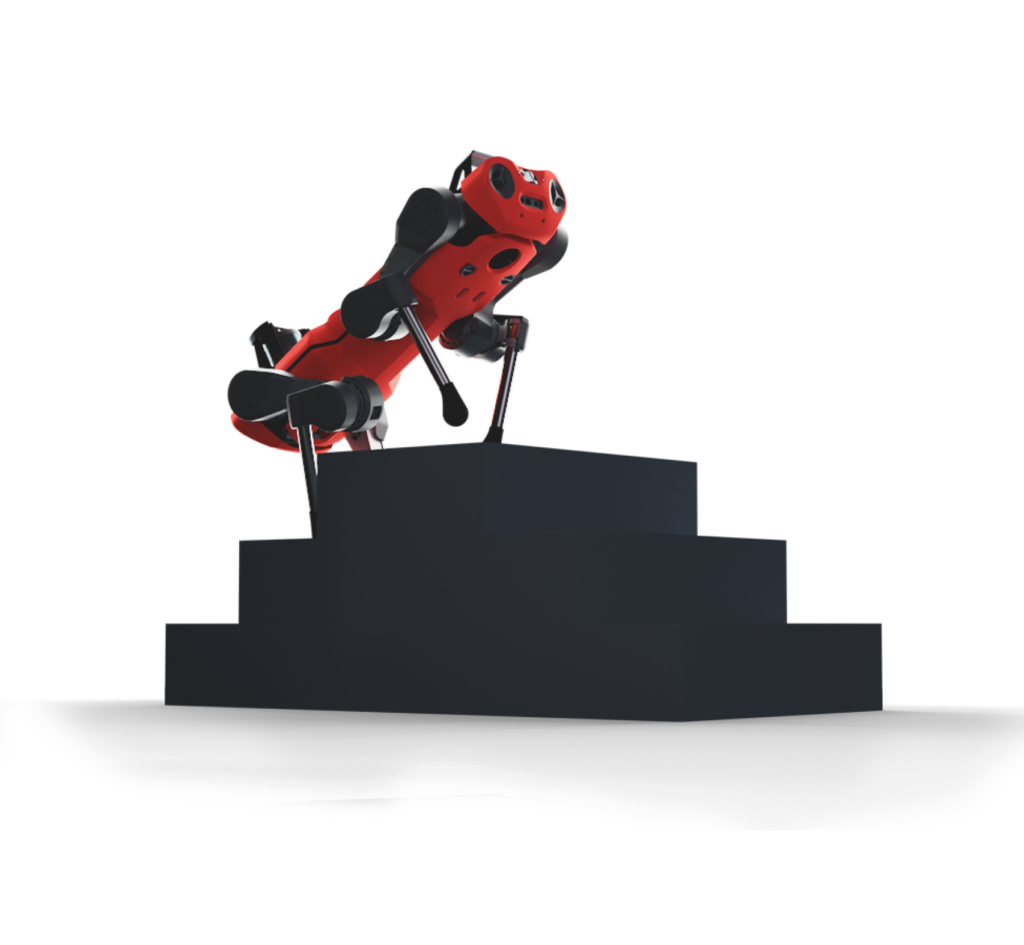
\includegraphics[width=1\textwidth]{./images/ANYmal.png}}}
        {https://www.anybotics.com/anymal-legged-robot/}
    \end{minipage}
    \begin{minipage}{0.7\textwidth}
            \textcolor{purple}{\textbf{Learning to Walk via Deep Reinforcement Learning}}:
            \begin{itemize}
                \item MDPs:  Markov Decision Processes
            \end{itemize}
            MDP Problem Formulation $\langle \mathcal{S, A, T, R}, \gamma \rangle$.

            \begin{figure}
                \cpright{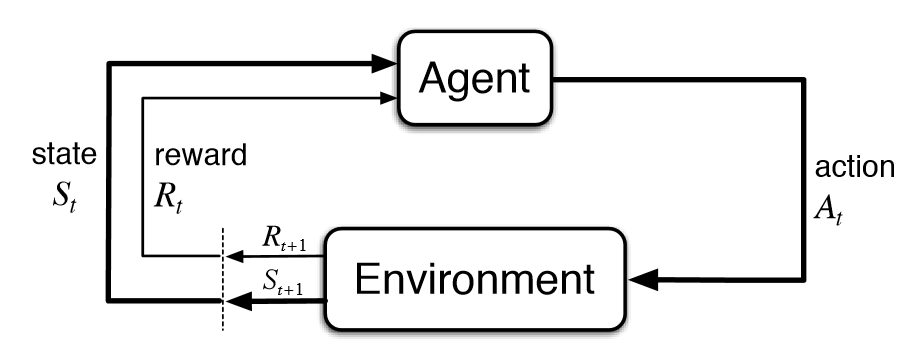
\includegraphics[width=0.8\textwidth]{./images/rl_diagram.png}}
                {}
            \end{figure}
    \end{minipage}
    \href{https://leggedrobotics.github.io/rl-blindloco/}{\small(ANYmal Learning to walk)}
    \href{https://www.youtube.com/watch?v=lKYh6uuCwRY}{\small(\faPlay Learning to walk)}
\end{frame}




\begin{frame}[fragile]{Modern Robots}
    \framesubtitle{ROS Packages for CHAMP Quadruped Controller}
        \begin{figure}
            \cpright{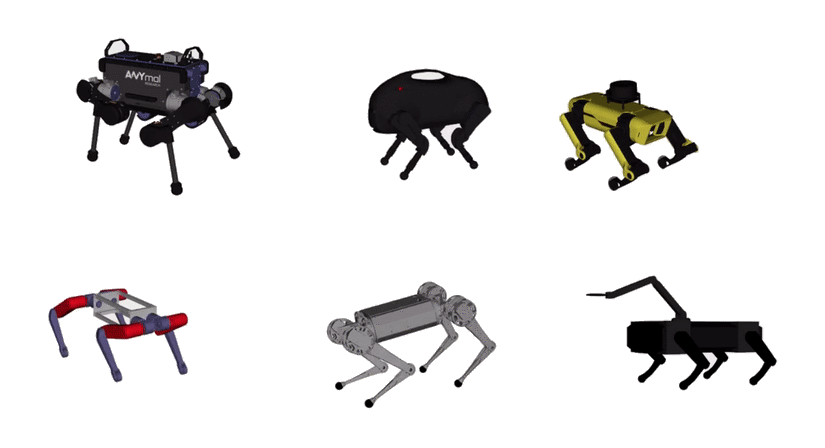
\includegraphics[width=0.8\textwidth]{./images/champ.png}}
                {https://github.com/chvmp/champ}
        \end{figure}
\end{frame}

\begin{frame}[t, allowframebreaks]
	\frametitle{References}
	\bibliography{\RMHOME/references.bib}
\end{frame}

\end{document}
